\documentclass[conference]{IEEEtran}
% *** MISC UTILITY PACKAGES ***
\usepackage{xcolor}
\usepackage{multirow}
% *** GRAPHICS RELATED PACKAGES ***
%
\ifCLASSINFOpdf
  \usepackage[pdftex]{graphicx}
\else
  \usepackage[dvips]{graphicx}
\fi

% *** MATH PACKAGES ***
%
%\usepackage[cmex10]{amsmath}

% *** ALIGNMENT PACKAGES ***
%
%\usepackage{array}

% *** SUBFIGURE PACKAGES ***
\ifCLASSOPTIONcompsoc
    \usepackage[caption=false,font=normalsize,labelfont=sf,textfont=sf]{subfig}
\else
    \usepackage[caption=false,font=footnotesize]{subfig}
\fi

%\usepackage[caption=false]{caption}
%\usepackage[font=footnotesize]{subfig}
%
\usepackage{url,hyperref}
\usepackage{float}
\usepackage[ruled,vlined]{algorithm2e}
\usepackage{amsmath}

% correct bad hyphenation here
\hyphenation{}


\begin{document}
%
\title{MPI solution for Fully Connected Neural Networks}

\author{
    \IEEEauthorblockN{Luiz F. M. Pereira}
    \IEEEauthorblockA{
        Department of Informatics\\
        State University of Maringá\\
        Maringá, Brazil\\
        \href{malito:ra103491@uem.br}{ra103491@uem.br}
    } 
}

% make the title area
\maketitle

\begin{abstract}
\boldmath
The use of neural networks in the area of pattern recognition has become increasingly common, however, to be effective, these networks require a large amount of processing. With the objective of reducing the execution time of an instance of the Fully Connected Neural Network, this paper proposed two different models of paralysis, with the use of shared memory and MPI. To test the effectiveness of the models, we tried to recognize numeric characters, from zero to nine, using the MNIST database. The test case that presented the highest speedup was the one that used all images, both training and test, and four processes, being equal to 4.08. Despite the good results for four processes, the speedup for two processes are very distanced from the expected, taking almost the same time as the sequential execution.
\end{abstract}

\begin{IEEEkeywords}
distributed programming, neural networks.
\end{IEEEkeywords}

\IEEEpeerreviewmaketitle

\section{Introduction}
% apresentar problema
Over the last several years, machine learning techniques, particularly when applied to neural networks, have played an increasingly important role in the design of pattern recognition (PR) systems. PR problems are often characterized by large and redundant training sets with high dimensional inputs, which translates into large networks and long learning times. One of the main contributions of Neural Networks to PR has been to provide an alternative to design properly. Multi layer networks can learn complex mappings in high dimensional spaces without requiring complicated handcrafted feature extractors \cite{lecun1995pattern}.

One of these neural networks is Fully Connected Neural Network (FCNN), a neural network model in which the adjacent network layers are fully connected to each other. As stated earlier, the training process in neural networks is very time consuming, a way to reduce this time is through paralysis of the process. One way to accomplish this parallelization is to use shared memory. This task can be done by using already established standards, such as MPI.

% falar do mpi
Message Passing Interface (MPI) is a standard message passing interface for distributed memory concurrent computers and networks of workstation \cite{the1993mpi}. The message passing paradigm is the most generally applicable and efficient programming model for parallel machines with distributed memory and has been used widely in parallel and distributed computing systems for some years \cite{clarke1994mpi}.
% contribuicao
In this paper, two solution to implement a FCNN in parallel is introduced. For this solution, the use of shared memory was chosen, which is managed by the MPI to C library, called OpenMPI. In the best scenario, it was possible to achieve a speedup equal to 4.08, using four processes and the largest input available.
% organizacao do artigo
This paper is organized as follows: in the next section we present the basic definitions about FCNNs; then we present our proposal to carry it out in parallel. In Section \ref{sec:settings} we present the tools used and the environment where the tests were carried out. In Section \ref{sec:analysis} we present the results obtained and analyze them in relation to performance and the impact of MPI instructions in code.

\section{Fully Connected Neural Networks}\label{sec:fcnn}

A Fully Connected Neural Network (FCNN), also called a Dense Neural Network (DNN) in data science, corresponds to the neural network model in which the adjacent network layers are fully connected to each other. Each neuron in the network is connected to each neuron in adjacent layers. To ensure that this definition is understood correctly by the reader, we present below some basic concepts related to neural networks \cite{kononenko2007machine}.

A neuron is a basic unit of a layer in FCNN. A neuron performs the multiplication and addition of weights to the input, similarly to linear regression, and the result is passed to the activation function. An activation function is responsible for defining the output of a neuron given a set of input data, some common examples are the Linear, ReLU and Sigmoid functions \cite{kononenko2007machine,alom2019state}.

It is possible to divide the use of neural networks into two different moments, the training and the test. The first consists of searching for optimization parameters (weights and bias) under the given network architecture and minimizing the classification error or residuals. This process includes two parts: feed forward and back propagation. The forward feed traverses the network with the input data (as forecast parts) and then calculates the loss of data in the output layer by loss function (cost function). After obtaining data loss, it is necessary to minimize data loss by changing weights and bias, a very popular method for this is to back-propagate the loss into every layers and neurons by gradient descent\footnote{\url{https://cs231n.github.io/convolutional-networks/}}. The number of times this process will be performed is called an epoch.

In this type of architecture, we can classify the layers in 3 categories: input layer, hidden layer and output layer. 

The input layer is generally fixed, with only one layer, and the number of nodes corresponds to the number of input features, in a scenario where images are used, the number of pixels in the image would define the number of nodes needed.

The nodes in the output layer generally do not have an activation because it is commonly used to represent the scores of each class in the classification. For classification, the number of output nodes corresponds to the number of classes to be forecasted.

The hidden layers are diverse, both in relation to the activation function used and the number of neurons used, and are the main component of an FCNN. In general, as the complexity of the problem grows, more hidden layers are needed to capture the desired patterns \cite{kononenko2007machine}.

To carry out the investigations proposed for this paper, the following architecture was chosen: one layer for input, one layer for output and 4 hidden layers. As the scenario chosen for tests was the classification of digits from 0 to 9, the input corresponds to an image, thus, the input layer has height x width nodes. Next we have 4 hidden layers, the first with 1024 neurons, in sequence we have the layers with 512, 256 and 10 neurons, in that order. For all hidden layers, the chosen activation function was ReLU, with the exception of the last layer used as Sigmoid as an activation function. Finally, the output layer has ten neurons, equivalent to the number of available classes. The architecture described is represented graphically in Figure \ref{fig:arq}.

\begin{figure}
    \centering
    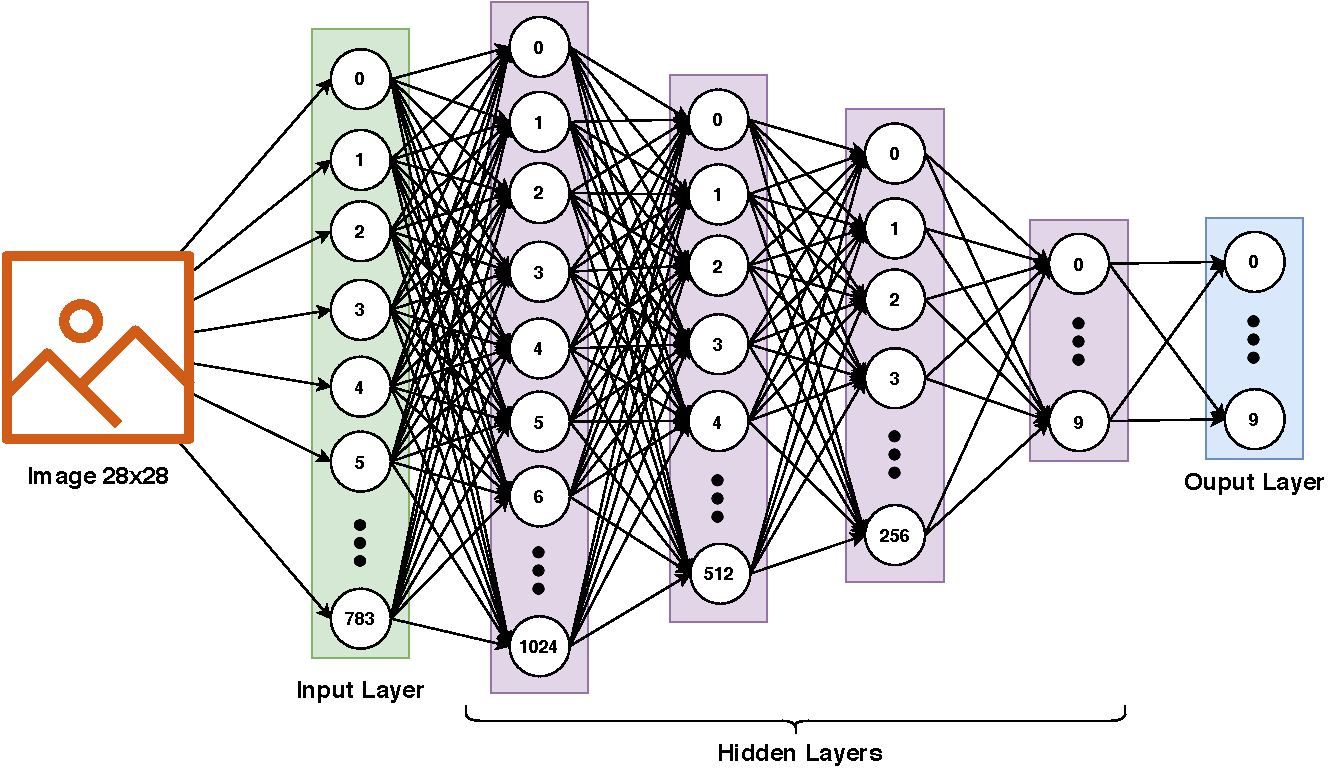
\includegraphics[width=\columnwidth]{images/FCNN.pdf}
    \caption{FCNN with four hidden layers}
    \label{fig:arq}
\end{figure}

Once created, the network is fed with each image and each layer performs forwarding, after that, the loss is calculated. When performing the loss calculation with the Mean Squared Error (MSE)\cite{lehmann2006theory}, it is necessary to do back propagation and update the weights for each layer.

With the training carried out, the test begins by means of forwarding, in which, when arriving at the output layer, a forecast for that image is obtained and verified with the label. If the forecast is different from the label, the loss is increased by one unit and the entire process is restarted and repeated until the number of epochs.

\section{MPI Solution}\label{sec:mpiversion}

Transforming the sequential version in parallel, using distributed memory, is very simple if we use MPI. Simply distribute the set of images between the processes and add barriers after reading the image, after training and after the test is completed. Let's look at the reason for using each one.

A barrier after image reading is necessary because only the master process performs this task, so other processes must wait for him to finish. After this barrier, the image data is transmitted to all other processes, through broadcasting, so that they have a copy of all training and test images.

The second barrier, right after the training is justified by the fact that it is not possible to proceed to the test stage without having even completed all the training. The training process, in turn, is performed only by the master process, as it updates the MSE error at each failure in the forecast, which must be done sequentially.

The last barrier ensures that all processes have already carried out the training and testing for that epoch and we are ready to update the weights and biases of the network. This update is done using reduce with all copies of each layer, that is, all the weights of each layer are added and the value obtained becomes the set of weights for all layers, this same operation happens for the biases of each layer.

Unfortunately, if the objective is to achieve the same accuracy with less time, just distributing images between the processes would not be enough. This happens because by maintaining several copies of the networks, we increase the randomness factor of the network, which contributes to the increased accuracy obtained. Thus, we proposed two modifications in the architecture to obtain an accuracy similar to that obtained in the sequential, however with a reduced time. To ensure that accuracy was not impaired, empirical tests were performed for each proposed modification.

The first modification, which we will call Model 1, seen in Figure \ref{fig:arqp1}, removes the last two hidden layers from the sequential architecture, keeping only the layer with 1024 and the layer with 512 neurons as hidden layers. The second modification, which we will call Model 1, seen in Figure \ref{fig:arqp2}, removes only the last hidden layer of the sequential architecture, with 10 neurons. Only the modifications are small, the difference produced in the speedup is considerable, as can be seen in Section \ref{sec:analysis}.

\begin{figure}
    \centering
    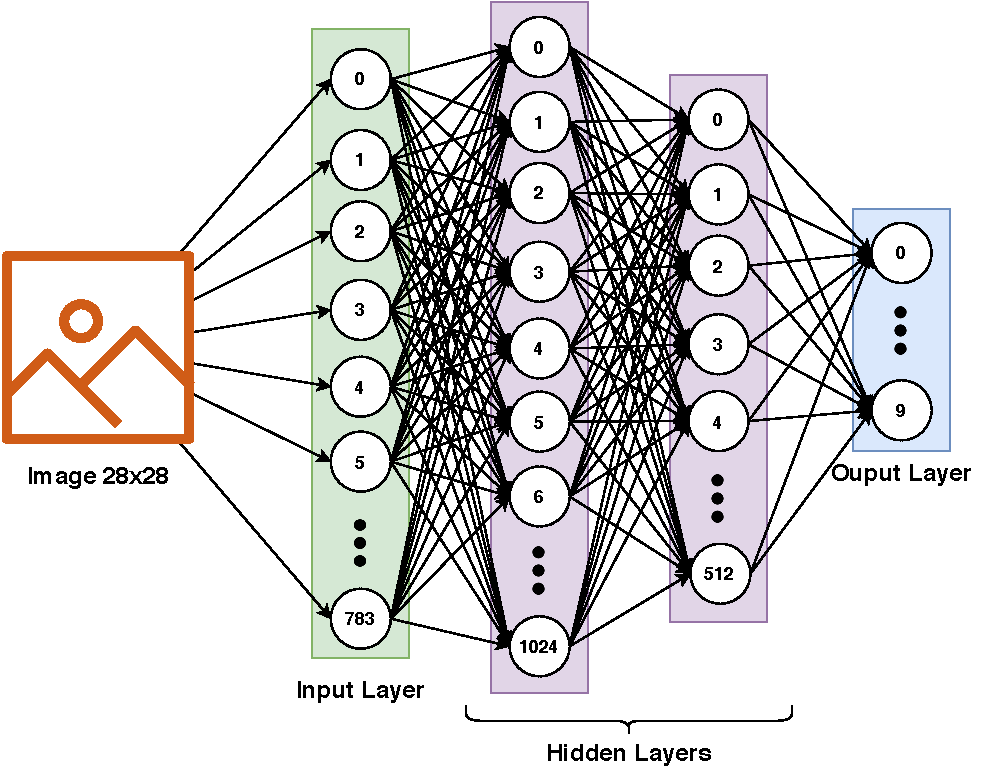
\includegraphics[width=\columnwidth]{images/FCNN-P1.pdf}
    \caption{FCNN with two hidden layers.}
    \label{fig:arqp1}
\end{figure}

\begin{figure}
    \centering
    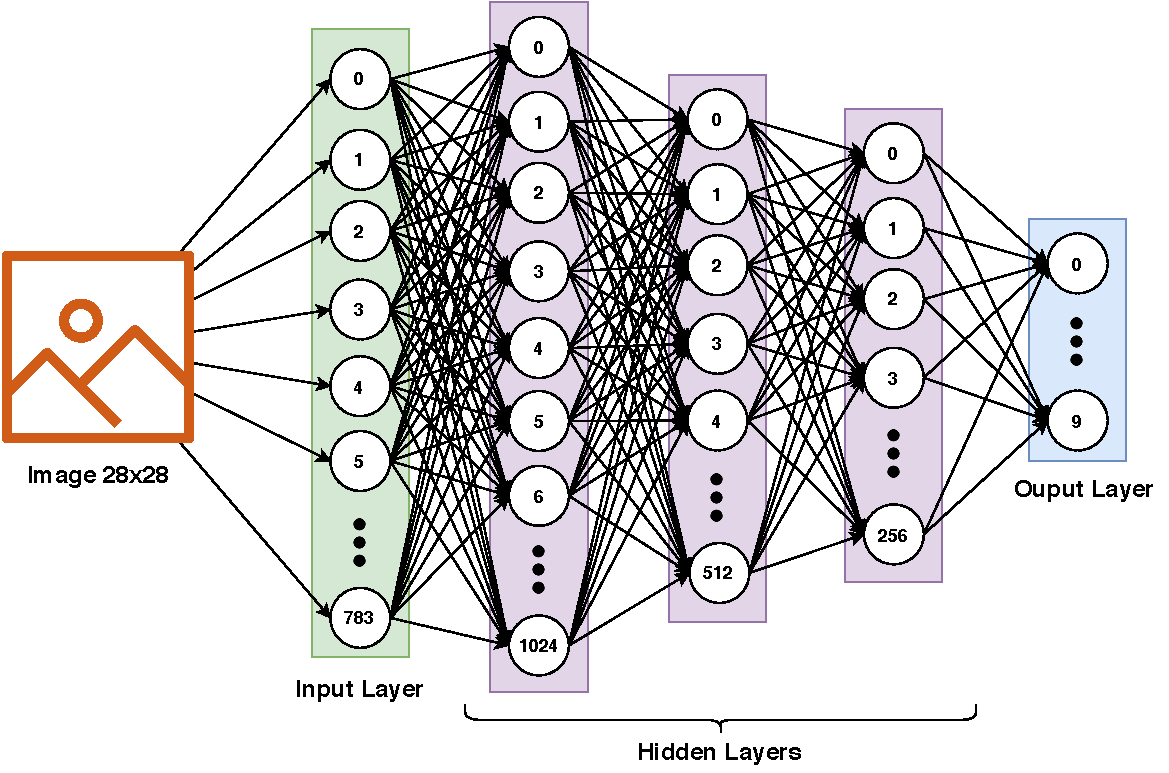
\includegraphics[width=\columnwidth]{images/FCNN-P2.pdf}
    \caption{FCNN with three hidden layers.}
    \label{fig:arqp2}
\end{figure}

\section{Experimental Settings}\label{sec:settings}

In this section, we detail the environment used for sequential and parallel execution. Following, we describe some details of the tools used for watch hardware events, for example, the number of messages sent, and measure performance, in subsection \ref{subsec:perftools}.

\subsection{Environment and Limitations}\label{subsec:env}

To carry out the experiments, all codes were developed using the C language and executed on the same machine. The select machine has Arch Linux, with kernel Linux 5.4.75-1-lts, as OS; Awesome as Windows Manager(WM), without desktop environment, GCC version 10.2.0 as compiler and Open MPI in version 4.0.5 to run MPI code. The machine's hardware configurations can be seen in the Table \ref{tab:pc-config}.

\begin{table}
\caption{Hardware specifications of the machine responsible for carrying out the tests.}
\centering
\begin{tabular}{cc}
\hline
\textbf{Hardware} & \textbf{Specification}                   \\ \hline
Model             & Notebook Dell G3 3590                    \\
Processor         & Intel(R) Core(TM) i5-9300H CPU @ 2.40GHz \\
Physical Cores    & 4                                        \\
Thread by core    & 2                                        \\
L1d cache         & 32 KB                                    \\
L1i cache         & 32 KB                                    \\
L2 cache          & 256 KB                                   \\
L3 cache          & 8192 KB                                  \\
Cache line size   & 64 b                                     \\
RAM Memory        & 8 GB                                     \\
Swap partition    & 15 GB                                    \\ \hline
\end{tabular}
\label{tab:pc-config}
\end{table}

% falar da temperatura
Considering that the machine used is a notebook, the results are expected to suffer interference in relation to performance. Since in this type of equipment the cooling system is weakened and the focus is on energy savings, the Operational System (OS) often tends to take more drastic measures in relation to the scheduling and freeze of processes.

\subsection{Performance Analysis Tools}\label{subsec:perftools}

In order to compare the performance of the sequential algorithm with its parallel version, two tools were used. The first tools is the Perf\footnote{\url{https://perf.wiki.kernel.org/index.php/Main_Page}} program, used to extract relevant data about the hardware and software events that occurred during the execution.The second tool is called mpiP\footnote{\url{https://software.llnl.gov/mpiP/}} and is used to collect statistical information about MPI functions.

Perf is an event-based analysis, monitoring and debugging tool, that is, events must be predefined in order to be able to collect and process them during the analysis process. Measurable events at Perf are from different sources, are present in most components of the kernel and hardware. It is worth mentioning that the event monitoring has limitations, whether in terms of accuracy or number of events available for the chosen processor \cite{weaver2013linux}.

According to the project's authors, mpiP is a lightweight profile library for MPI applications and generates considerably less overhead and much less data than tracking tools, as well as merging results from all tasks into one output file.

\section{Analysis and Discussion}\label{sec:analysis}

In this section we present some information about the results obtained and what we can conclude about them. First we present an analysis of the performance through the Speedup metric, then we analyze the impact of MPI functions call in execution time.

\subsection{MNIST Database}\label{subsec:test}
To carry out the tests on the models built, the MNIST database\footnote{\url{http://yann.lecun.com/exdb/mnist/}} was chosen and different quantities of samples were used, having 16 epochs as a standard. The MNIST database of handwritten digits has a training set with 60,000 examples and a test set with 10,000 examples. The digits were normalized in terms of size and centered on a fixed size image, 28 pixels high by 28 pixels wide. An example of the base samples can be seen in Figure \ref{fig:mnist}. It is a good database for people who want to try learning techniques and pattern recognition methods on real-world data while spending minimal efforts on preprocessing and formatting\footnote{The database can be downloaded at the following link: url{https://drive.google.com/file/d/1alUM0B0PtYLTw4TWUNMyByIxyZn81FYO/}}.

\begin{figure}[H]
    \centering
    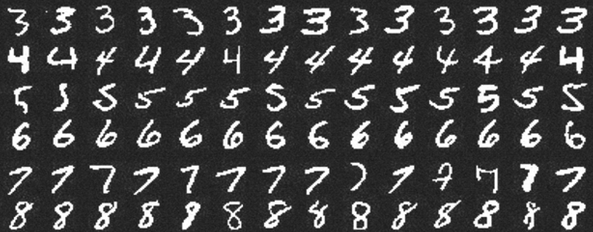
\includegraphics[width=\columnwidth]{images/mnist-example.png}
    \caption{Example of samples from MNIST database.}
    \label{fig:mnist}
\end{figure}

\subsection{Speedup}
% definicao
One of the goals of parallelizing an application is to decrease the execution time. A way to tangibly compare the performance of a sequential application with its parallel version, in relation to time, is to calculate the Speedup. The Speedup metric can be calculated by the ratio of serial execution time to parallel execution time. For an application with good scalability, the speedup should, ideally, increase at the same rate as the increase in the number of processes.

% falar do problema da sincronizacao
Although we want Speedup to be always linear, this is not always the reality. In line with Amdahl's law\cite{schmidt2017parallel}, we have to, the speedup of a parallel program is limited by the time needed to compute the sequential fraction of that same program, this implies that in these types of problems the ideal Speedup will hardly be reached.

% falar dos casos testados
To guarantee the effectiveness of the parallelism with MPI, tests with four different input sizes were carried out for both proposed modifications. Due to the limitations in the amount of physical cores of the test machine, only four, the inputs were tested only for two, three and four processes. We will define the entries as follows: 1000 images for training and 300 images for testing; 9000 images for training and 3000 images for testing; 30000 images for training and 6000 images for testing; finally, 60000 images for training and 10000 images for tests will be called \textit{small}, \textit{medium}, \textit{large} and \textit{extra large}, respectively.

% falar dos resultados e explicar
First, it is important to note that the time used to calculate the speedup werethe overall average time of ten runs, ie, they include the reading time of the images and labels. As expected, as we increase the amount of hidden layers the speedup drops, as it is possible to verify by comparing Figures \ref{fig:speedup1} and \ref{fig:speedup2}. It is worth remembering that, although Model 1 has a shorter execution time, Model 2 is the one who tends to present greater accuracy. Thus, the choice of which model to use will depend on the programmer's need.

It is also possible to observe that the performance for two processes had the result much below the ideal for both models. Several may be the reasons why this has occurred, we can cite as an example the amount of time required to perform the broadcast and reduce the data, however, to discover and overcome all obstacles that prevent the model to approach the ideal result, it would be necessary to run other performance analysis tools that would provide a broader amount of data on execution.

Despite the performance far from ideal for two and three processes, for four processes the speedup obtained was satisfactory, given that the problem is not embarassingly parallel, even reaching the linear speedup for the extra large entry. This result can only be obtained thanks to the modifications made to the sequential model, because, as stated before, when the amount of hidden layers increases, the speedup tends to decrease.

\begin{figure}
    \centering
    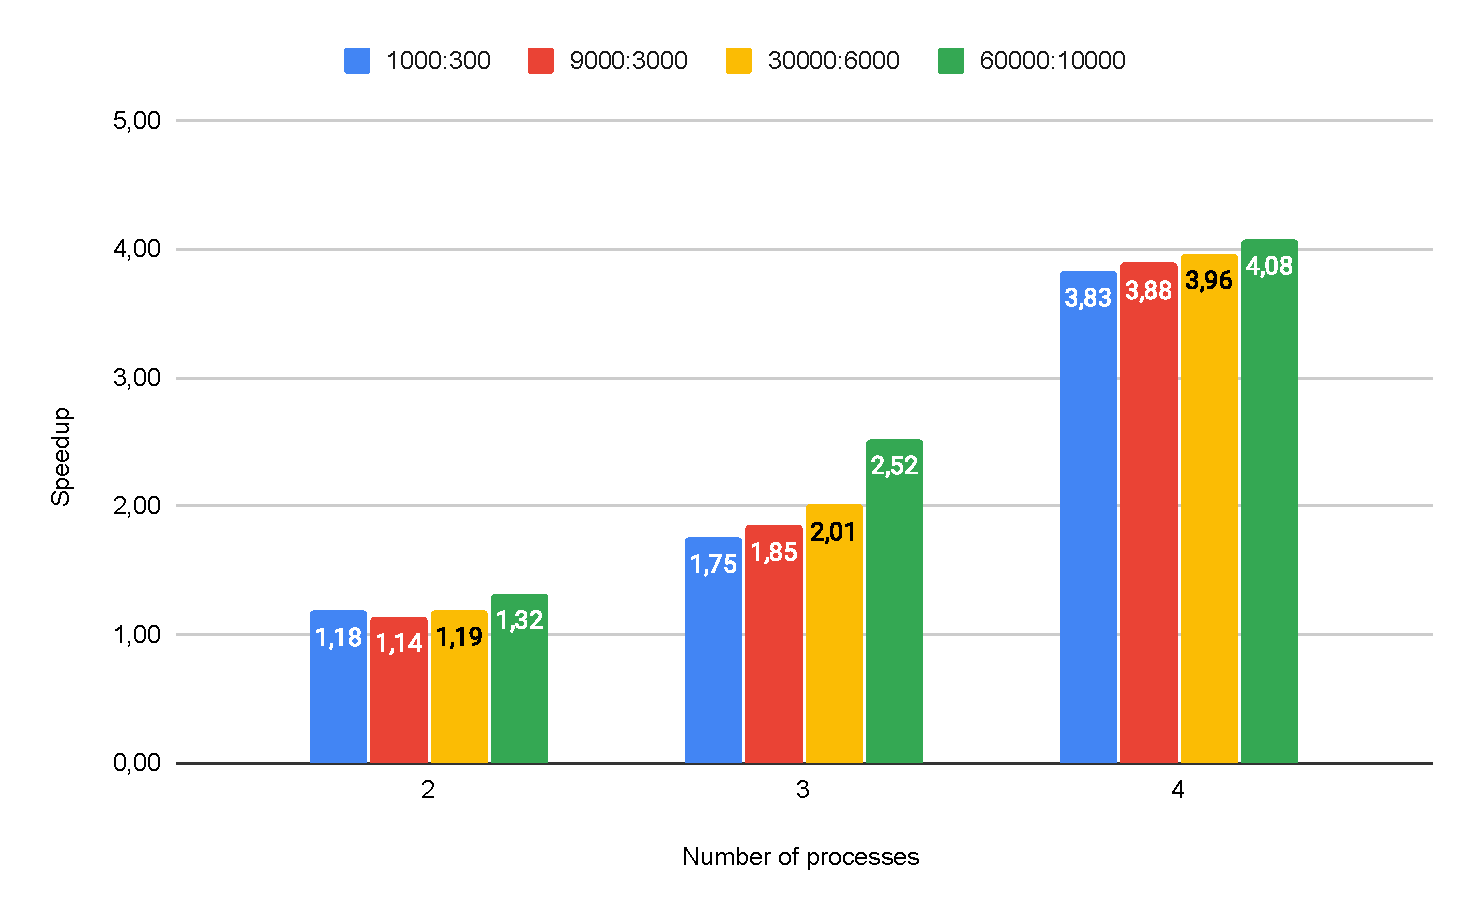
\includegraphics[width=\columnwidth]{images/speedup-model1.pdf}
    \caption{Model 1 speedup for 2, 3 and 4 processes.}
    \label{fig:speedup1}
\end{figure}

\begin{figure}
    \centering
    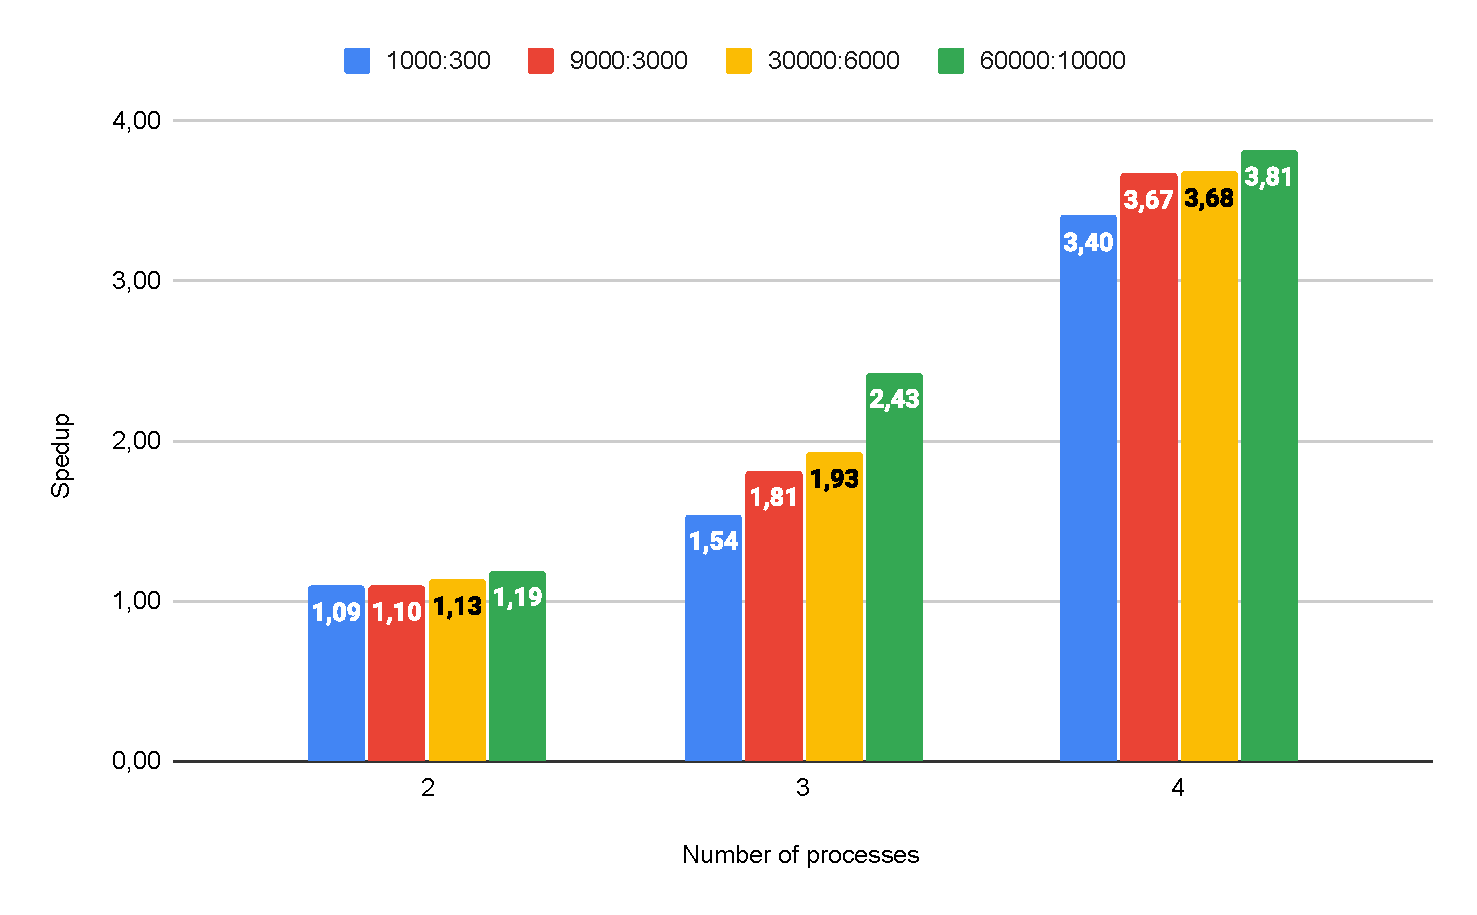
\includegraphics[width=\columnwidth]{images/speedup-model2.pdf}
    \caption{Model 2 speedup for 2, 3 and 4 processes.}
    \label{fig:speedup2}
\end{figure}

\subsection{MPI impact}

In exchange for a parallel execution, there are costs in relation to sending and receiving data, barriers, etc, which must be paid when using MPI. In the proposed models of FCNN, as the number of processes increases, the time spent with functions of the MPI library increases. This behavior is justified by the fact that each process must have a copy of all the training and test images, that is, the more processes, the greater the amount of messages that are trafficked.

Note, however, that, in relation to the total time, these costs are decreasing in relation to the size of the input grows, that is, for the same amount of processes, the greater the size of the input, the less expressive the percentage of time spent with intrinsic functions of MPI. This behavior can be clearly seen in Figure \ref{fig:mpimaxtime}, which shows the time, in percentage, spent only with the operations of the MPI library for Model 1.

\begin{figure}
    \centering
    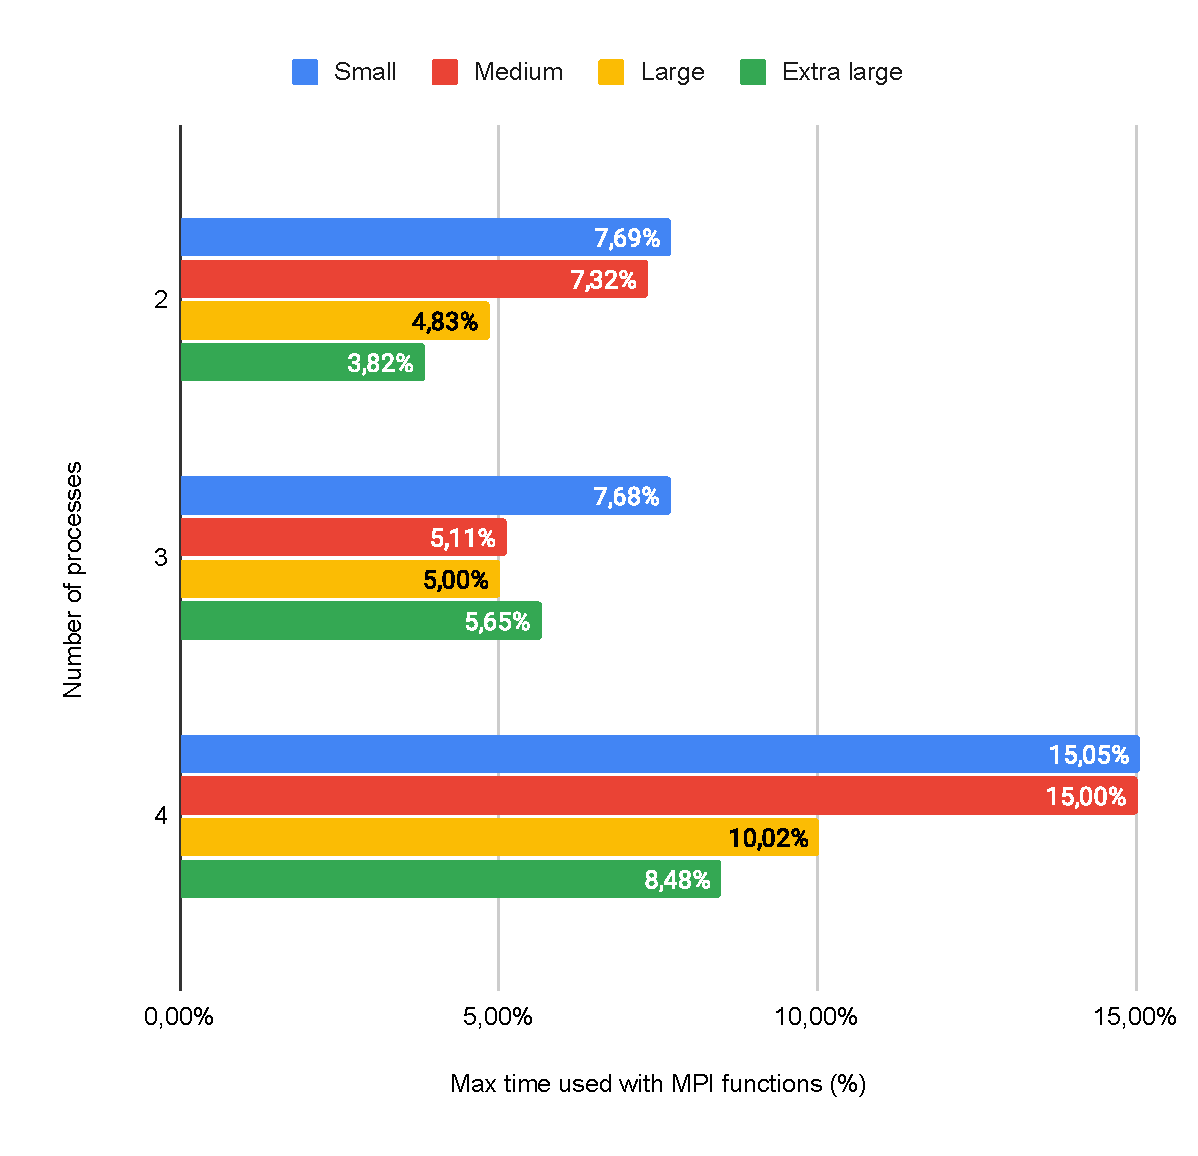
\includegraphics[width=\columnwidth]{images/mpi-max-time.pdf}
    \caption{Max time used with MPI functions for Model 1.}
    \label{fig:mpimaxtime}
\end{figure}

The same behavior can be observed for Model 2 in Figure \ref{fig:mpimaxtime2}. Note, however, that the percentage of time spent with the same operations in Model 2 is lower compared to the previous one, for two and four processes, this fact is probably linked to the addition of a layer in relation to Model 1, which implies a greater amount of messages to be trafficked, since the number of copies to be made available also increases.

\begin{figure}
    \centering
    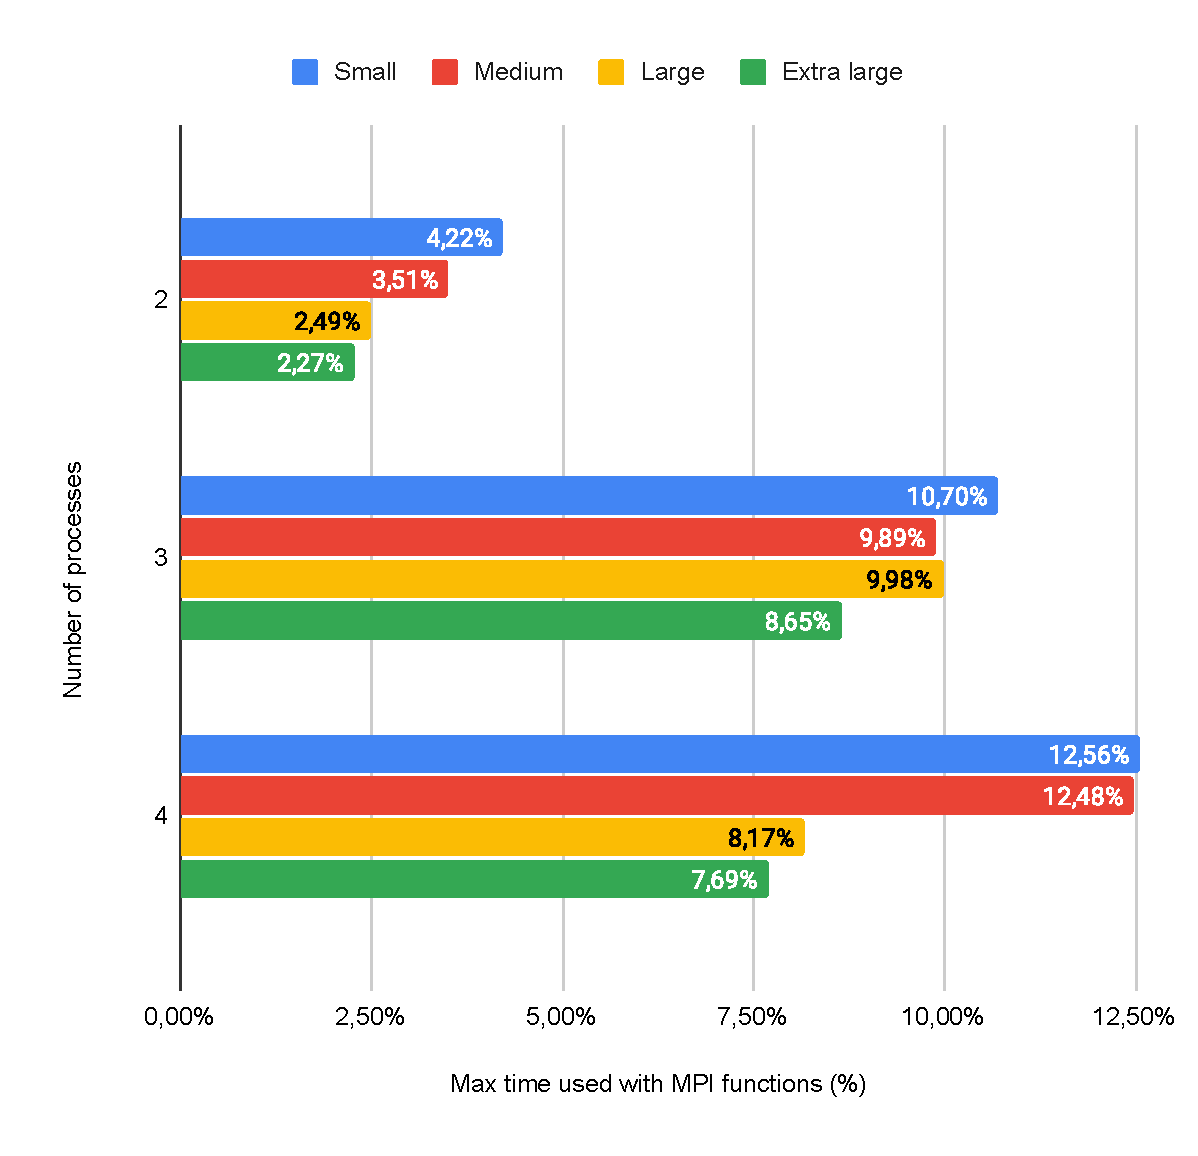
\includegraphics[width=\columnwidth]{images/mpi-max-time-m2.pdf}
    \caption{Max time used with MPI functions for Model 2.}
    \label{fig:mpimaxtime2}
\end{figure}

\section{Concluding Remarks}
FCNNs are highly generic models and can be used for pattern recognition, optimization, data generation tasks, etc. In this paper, we compare three different implementations of this neural network model, one of which is the sequential model and the other two, models that use shared memory through MPI. The maximum speedup obtained was 4.08, achieved in tests with four processes and using 60,000 training images and 10,000 test images. Unfortunately, the results for two processes were far from expected. As future work, investigations will be carried out to find out what caused the model's low performance for lower process values. In addition, it is intended to implement new variations to the model in order to achieve greater accuracy with less execution time.
\bibliography{references.bib}
\bibliographystyle{IEEEtran}
% that's all folks
\end{document}


